\chapter{Design}
\label{chapter: 4}

This chapter describes the development tools that the project used and then gives an overview of the system before detailing in the algorithms that the solution will use as well as justifying why they are used. 

\section{Development Tools}

The system is built using ROS, which provides frameworks for robot software development. ROS supports C++ and Python, with the project using Python due to experience and a faster development time. The system also uses the MiRo Development Kit (MDK) which provides useful functions for interfacing with the MiRo, such as retrieving data from the camera and current pose estimation.

The project was developed in simulation first before being tested on real robots due to the limited availability of the MiRos. Evaluation is also done in simulation as the actual position of the ball can easily be accessed and compared to the observed position. The Gazebo simulator was chosen as MiRo already has support and it has useful features such as a physics engine and integration with ROS.

Numpy is a python library that offers a large collection of mathematical functions implemented in C, meaning that computation can be much more efficient than in pure python, which is very useful for projects with limited processing power such as this one. The python libraries scikit-learn and scikit-image are also used in the project, the former providing implementations for machine learning models such as the support-vector machine classifier and the latter providing image processing algorithms such the histogram of oriented gradients feature descriptor. 

\section{System Overview}

The goal of the system is to provide information about the current and future state of the ball. The three key pieces of information are the current ball position, the current ball velocity and the predicted position of the ball some time in the future. 

The main loop runs at a rate of 10 ticks per second to keep a reasonably up to date estimate while leaving enough time to process the images. Ball position and velocity are published to a ROS topic on every tick and include a confidence value representing how likely the estimate is to be accurate. Ball trajectory is implemented as a ROS service that returns a position estimate at $t$ seconds in the future upon request.

\section{Image Processing}

\subsection{Camera Feed Parameters}

The first step of the process is to retrieve the images from the camera feed. An image size of 640x360 pixels is used as this provides sufficient detail for ball detection while being small enough to be processed in an acceptable time. The camera feed publishes images at a rate of 15Hz, however the system only runs at a rate of 10Hz as this allows enough time for the system to run consistently and is still sufficiently fast enough to react to the dynamic world. 

\subsection{Camera Calibration}

The cameras are calibrated using a dataset of chessboard images at various rotations and positions around the stationary cameras. Figure \ref{fig:camera calibration} shows how the size of the dataset affects the quality of the calibration measured using the re-projection error, for which value closer to zero represents a better calibration. A dataset of 16 images is used as this has the best performance across both cameras. 

\begin{figure}[H]
    \centering
    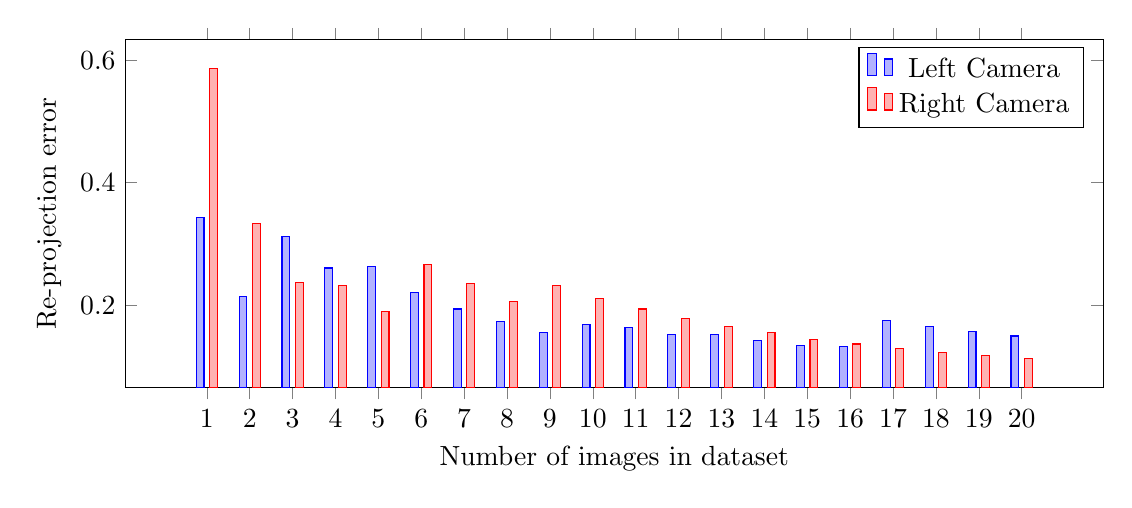
\begin{tikzpicture}
 
    \begin{axis} [ybar,
        height=6cm,
        width=14cm,
        bar width=0.1cm, 
        xlabel={Number of images in dataset}, 
        ylabel={Re-projection error},
        xtick={1,2,3,4,5,6,7,8,9,10,11,12,13,14,15,16,17,18,19,20}
        ]
     
    \addplot coordinates {(1, 0.343) (2, 0.214) (3, 0.312) (4, 0.261) (5, 0.263) (6, 0.221) (7, 0.194) (8, 0.173) (9, 0.156) (10, 0.169) (11, 0.164) (12, 0.153) (13, 0.153) (14, 0.143) (15, 0.135) (16, 0.133) (17, 0.175) (18, 0.166) (19, 0.158) (20, 0.150) };
    \addplot coordinates {(1, 0.586) (2, 0.333) (3, 0.237) (4, 0.232) (5, 0.190) (6, 0.266) (7, 0.235) (8, 0.207) (9, 0.232) (10, 0.211) (11, 0.194) (12, 0.178) (13, 0.166) (14, 0.155) (15, 0.145) (16, 0.137) (17, 0.129) (18, 0.123) (19, 0.118) (20, 0.113) };
     
    \legend {Left Camera, Right Camera};
     
    \end{axis}
 
    \end{tikzpicture}
    \caption{Analysing how the size of the dataset affects calibration quality}
    \label{fig:camera calibration}
\end{figure}

\section{Ball Detection}

After a calibrated image is retrieved, a decision must be made as to how to process the image in order to locate the position of the ball - or how to tackle the problem of object detection. A neural approach such as a convolutional neural network can produce very impressive results, however due to their computational complexity they are not appropriate for this project. This means that a non-neural approach must be taken. 

A common solution is to use a sliding window, classifying each area of the image to find the position of the ball. However this method requires hundreds or even thousands of areas to be classified meaning that a feature vector must be generated and evaluated for every area, which is a very computationally expensive process. This is not feasible for this project so a more efficient solution is required.

The method chosen can be broken down into two steps; an feature extraction algorithm to produce a list of potential ball candidates and a set of filters to remove false positives from this list.

\begin{figure}[H]
    \centering
    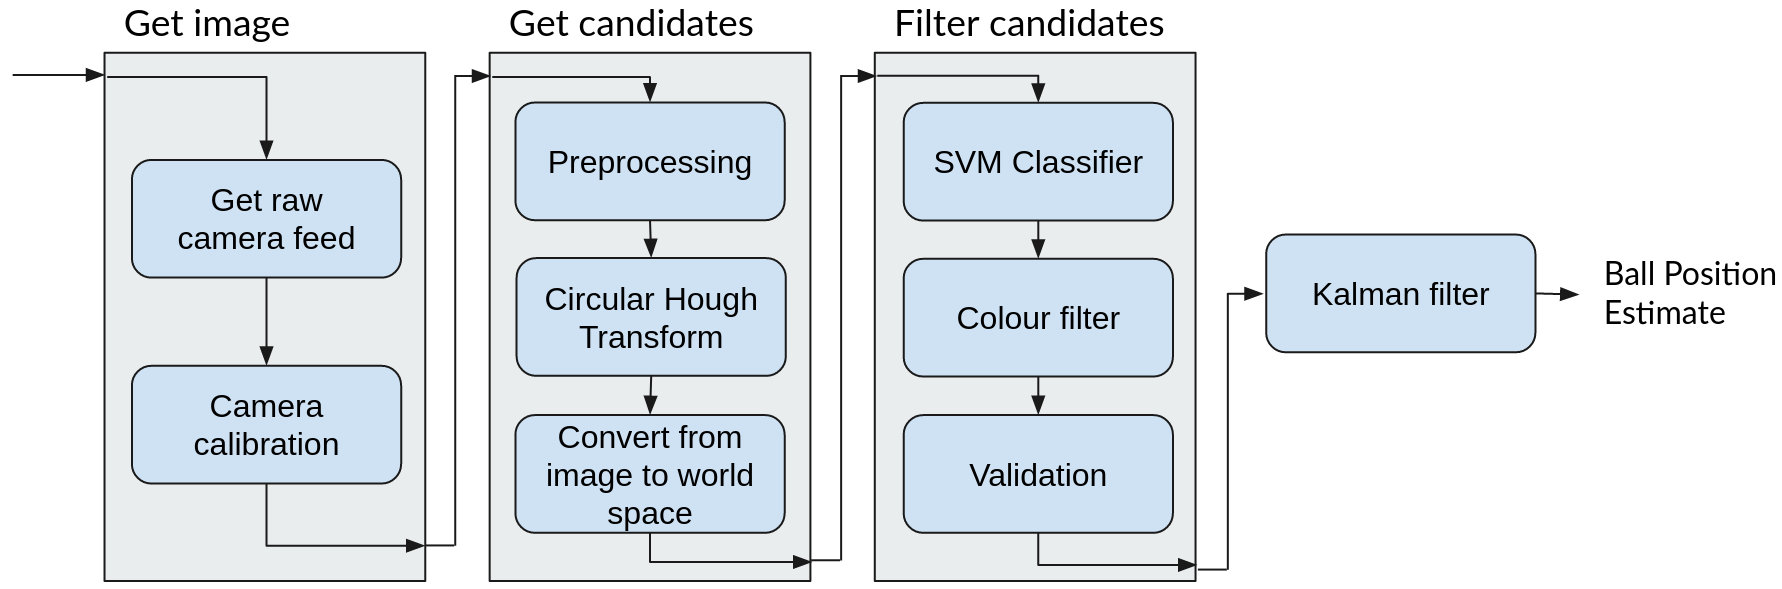
\includegraphics[width=16cm]{images/position-design.png}
    \caption{Flow diagram for ball position design}
    \label{fig:position design}
\end{figure}

\subsection{Get Candidates}

\subsubsection{Circular Hough Transform}
\label{section: Hough design}

The circular Hough transform is used to generate a list of ball candidates from the image. This algorithm was chosen for this task as it can produce reliable results very efficiently compared to alternative feature extraction techniques such as blob detection. However this efficiency comes at a cost of needing a well segmented mask, meaning that circular shapes have to be detected by colour. As well as decreasing robustness to changes in lighting and ball pattern, this requires that the ball is a different colour to the floor and walls of the pitch. 

\subsubsection{Preprocessing}

The raw camera feed must be converted to a mask so that the circular Hough transform can more reliably detect the ball. This mask is produced by colour segmentation. Any pixels that match the colours of the ball, or are within a range of these colours, are included in the mask while other pixels are discarded, resulting in a binary image. For this task the image is converted to the HSV colour space, which is preferred to RGB as it is easier to define ranges for the colour thresholding. This mask is then cleaned up using a Gaussian blur as well as erode and dilate operations to reduce noise.

\subsubsection{Image to World Space Conversion}

For this conversion there are three relevant spaces: image space, head space and world space. A position in image space is a 2-dimensional coordinate representing a pixel in the image, with the origin in the top left corner. A position in head space is a 3-dimensional coordinate representing the position of a point, relative to the transformation of MiRo's head. The origin of this space is equal to the position of the head. A position in world space is a 3-dimensional coordinate representing a point in the world, completely unrelated to the MiRo. This means that any position in image or head space is specific to one agent, whereas a position in world space can be understood by any agent.

To convert from image space to world space, the pixel coordinate is converted to a position in head space using an estimated distance of the ball. This is then converted to world space using information about the current robot kinematics and position in the world. 

\begin{figure}[ht]
    \begin{subfigure}[b]{0.4\textwidth}
        \centering
        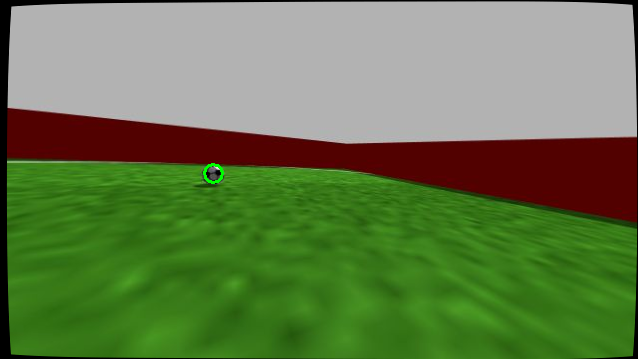
\includegraphics[width=6cm]{images/imagespace.png}
    \end{subfigure}
    %
    \begin{subfigure}[b]{0.4\textwidth}
        \centering
        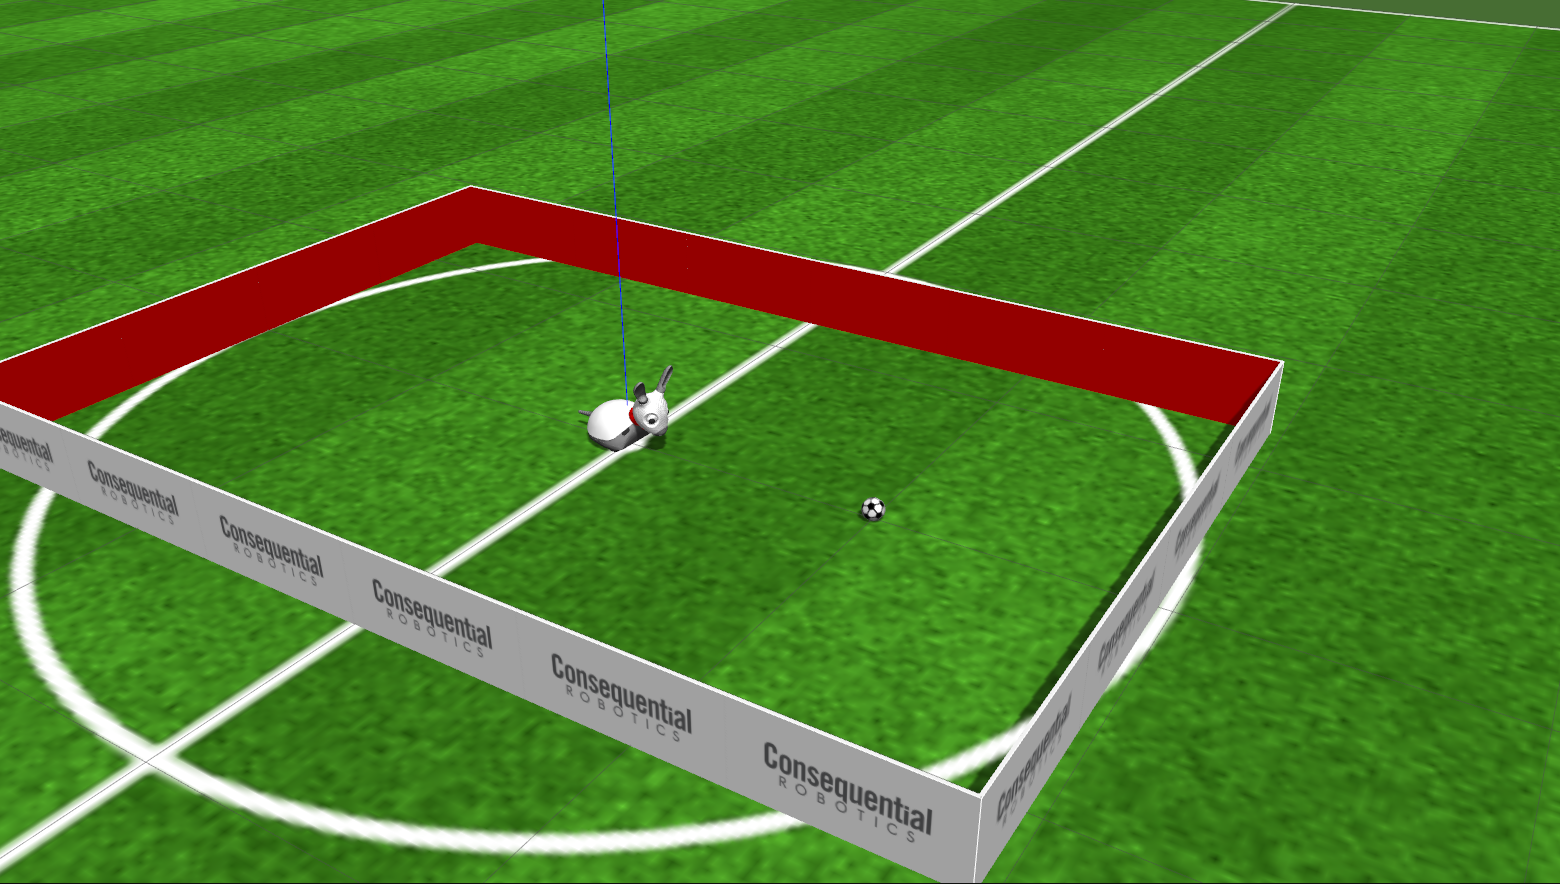
\includegraphics[width=6cm]{images/worldspace.png}
    \end{subfigure}
\centering

In this scenario, the ball is at $\begin{bmatrix}214 & 174 \end{bmatrix}$ in image space and $\begin{bmatrix}-1 & 0 & 0.04 \end{bmatrix}$ in world space. Therefore the position in head space is $\begin{bmatrix}1 & 0 & -0.2 \end{bmatrix}$. The $x$ value is positive as the MiRo is facing the ball and the $z$ value is negative as the ball is below the height of the head.
\caption{Illustrating image space and world space}
\end{figure}

\subsection{Filter Candidates}

\subsubsection{SVM Classifier}
\label{section: svm-hog}

The primary filter is a classifier that evaluates whether an area of the image is a ball. The classifier uses the histogram of oriented gradients (HOG) feature descriptor to summarise the shape information of the area. HOG is preferred to other feature descriptors such as SURF or SIFT as it is computationally efficient enough to run in real time and proven in object detection problems. A support-vector machine (SVM) is the favoured classifier as it is also well documented in this problem, especially in combination with the HOG feature, and was found to be more efficient than other options such as a decision tree classifier. Analysis of the performance of classifiers can be found in \ref{section: svm-implement}.

\subsubsection{Colour Filter}
\label{section: colour filter design}

The second filter takes advantage of the colour information of the image, using K-means clustering to extract the most common colours of the image. If these most common colours do not match that of the ball then the candidate can be rejected. The purpose of this filter is to reject candidates that have been missed by the classifier due to having a similar shape to the ball and to reject candidates that might contain the ball as well as a larger area surrounding it which could lead to inaccuracies in position estimation.

\subsubsection{Validation}

Some validation is performed on the candidates using their world positions. The first is to reject any candidates that are outside the borders of the pitch, although there is some leeway to allow for small errors in position when the ball is at the edge of the pitch. Another validation is to check that the candidate is not too far from previous estimates. This uses a normal distribution on the last 10 positions (approximately 1 second) as well as 5 future predictions at intervals of $1/10$ seconds to account for the expected movement of the ball. Any positions that are not within 3 standard deviations of this distribution are rejected. The last validation is to limit there to only be one candidate for each image. The best candidate is chosen by comparing the confidence value of classifier's evaluation.
 
 \subsection{Kalman Filter}
 
These final ball positions are then fed into a Kalman filter which uses a combination of a prediction model and perceived positions to output a best estimate of the current position of the ball in world space. The Kalman filter is favoured over other fusion techniques due to having good performance on kinematic problems like this one and its much greater computational efficiency than options such as Monte Carlo Localisation. 

The filter uses the state vector

\[\hat{x}_{k|k} = \begin{bmatrix}position_x \\ position_y \\ velocity_x \\ velocity_y\end{bmatrix}\]

\noindent and the transition function

\[F_k = \begin{bmatrix} 1 & 0 & \Delta t & 0 \\ 0 & 1 & 0 & \Delta t \\ 0 & 0 & 1 & 0 \\ 0 & 0 & 0 & 1\end{bmatrix}\]

This assumes that the ball velocity is constant between updates, which is an acceptable assumption as there is a short time between updates (100ms) and noise in the data makes calculating any change in the velocity unreliable. 


\section{Ball Velocity}

\begin{figure}[H]
    \centering
    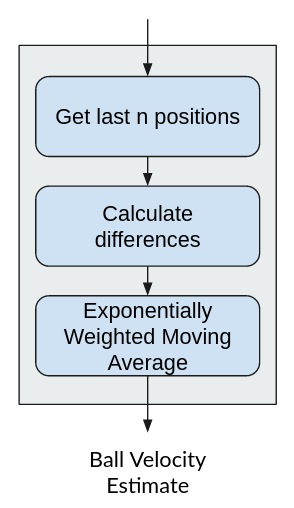
\includegraphics[width=4cm]{images/velocity-design.png}
    \caption{Flow diagram for ball velocity design}
    \label{fig:velocity design}
\end{figure}

Ball velocity is estimated using a list of the most recent ball position estimates. The difference between each adjacent position is calculated and an exponentially weighted moving average (EWMA) is performed on the differences to give an estimate for velocity. EWMA is chosen so that more recent values have a greater contribution to the average, meaning that the system can react to changes in velocity more quickly.

\section{Trajectory Prediction}

\begin{figure}[H]
    \centering
    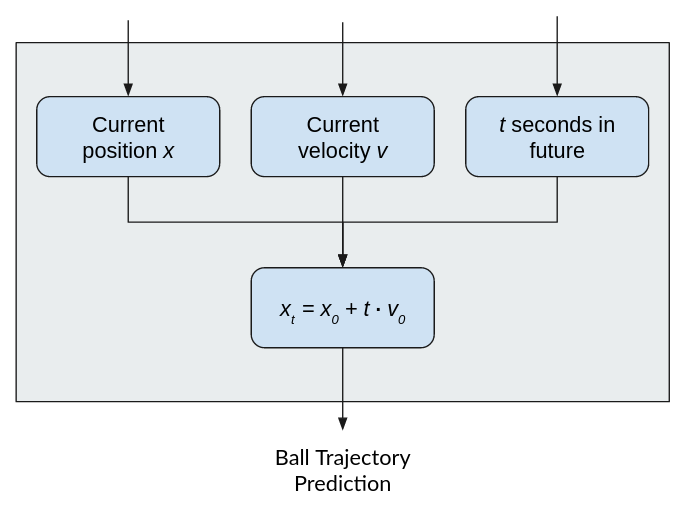
\includegraphics[width=9cm]{images/trajectory-design.png}
    \caption{Flow diagram for ball trajectory design}
    \label{fig:trajectory design}
\end{figure}

The trajectory of the ball is estimated using the kinematic equation:
\[ x_t = x_0 + t \cdot v_0 \]
Where $x$ is the future position, $x_0$ is the current position, $v_0$ is the current velocity and $t$ is the time in the future to estimate the position for. This method is used due to its simplicity, however a more advanced technique could provide more accurate results. 
